\documentclass{standalone}
\usepackage{tikz}
\usetikzlibrary{intersections,calc}
\usepackage{amsmath}
\usepackage{hsbcommon}
    \begin{document}
    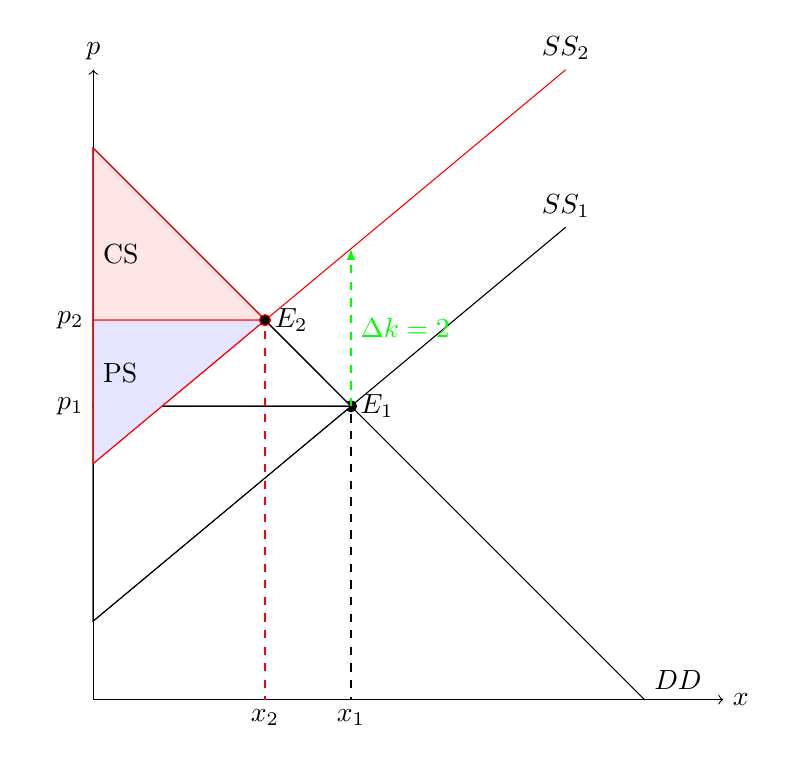
\begin{tikzpicture}
        \draw[->] (0,0) node[below] {\phantom{$X_mi$}} -- (8,0) node (Y) [right] {$x$};
        \draw[->] (0,0) node[left] {\phantom{$Y_mi$}} -- (0,8) node (i) [above] {$p$};

        
        
        \coordinate (A) at (0,7);
        \coordinate (B) at (7,0);
        \coordinate (E) at (0,1);
        \coordinate (F) at (6,6);
        
        \draw[name path=demand] plot [smooth] coordinates {(A) (B) };
        \node[above right] at (B) {$DD$};
        
        \draw[name path=supply] plot [smooth] coordinates {(E) (F)};
        \node[above] at (F) {$SS_1$};
            
        \path [name intersections={of=demand and supply,by=X}];
        
        \draw[dashed] (0, |- X) node [left] {$p_1$} -- (X) -- (X |-, 0)  node [below] {$x_1$}; 
        
        \draw[fill=red!10] (A) --  (X) --   (0, |- X) -- node[below right] {\parbox{13ex}{CS}} cycle;
        \draw[fill=blue!10] (E) --  (X) --   (0, |- X) -- node[above right] {\parbox{13ex}{PS}} cycle;
    
        \filldraw (X) node[right] {$E_1$} circle (2pt);

    \ifstep{2}{
\begin{scope}[draw=red]

        \draw[color=black,fill=white] (A) --  (X) --   (0, |- X) --  cycle;
        \draw[color=black,fill=white] (E) --  (X) --   (0, |- X) -- cycle;             
        
        \coordinate (A) at (0,7);
        \coordinate (B) at (7,0);
        \coordinate (E) at (0,3);
        \coordinate (F) at (6,8);

        \draw[dashed,->,>=latex,color=green] (X) -- node[right] {$\Delta k=2$} ++ (0,2);
        
        % \draw[name path=demand] plot [smooth] coordinates {(A) (B) };
        % \node[above right] at (B) {$DD$};
        
        \draw[name path=supply] plot [smooth] coordinates {(E) (F)};
        \node[above] at (F) {$SS_2$};
            
        \path [name intersections={of=demand and supply,by=X}];

        
        \draw[dashed] (0, |- X) node [left] {$p_2$} -- (X) -- (X |-, 0)  node [below] {$x_2$}; 
        
        \draw[fill=red!10] (A) --  (X) --   (0, |- X) -- node[below right] {\parbox{13ex}{CS}} cycle;
        \draw[fill=blue!10] (E) --  (X) --   (0, |- X) -- node[above right] {\parbox{13ex}{PS}} cycle;
    
        \filldraw (X) node[right] {$E_2$} circle (2pt);
     
    \end{scope}
}

            
    \end{tikzpicture}
\end{document}
